\documentclass[a4paper,14pt]{extreport}
	\usepackage[left=1.5cm,right=1.5cm,
	    top=1.5cm,bottom=2cm,bindingoffset=0cm]{geometry}
	\usepackage{scrextend}
	\usepackage[T1,T2A]{fontenc}
	\usepackage[utf8]{inputenc}
	\usepackage[english,russian,ukrainian]{babel}
	\usepackage{tabularx}
	\linespread{1.5}
	\usepackage{amssymb}
	\usepackage{fp}
	\usepackage{color}
	\usepackage{amsmath}
	\usepackage{mathrsfs}
	\usepackage{listings}
	\usepackage{graphicx}
	\graphicspath{ {./images/} }
	\usepackage{lipsum}
	\usepackage{xcolor}
	\usepackage{multirow}
	%\usepackage[table,xcdraw]{xcolor}
	\usepackage{hyperref}
	\usepackage{tcolorbox}
	\usepackage{tikz}
	\usepackage[framemethod=TikZ]{mdframed}
	\usepackage{wrapfig,boxedminipage,lipsum}
	\mdfdefinestyle{MyFrame}{%
	linecolor=blue,outerlinewidth=2pt,roundcorner=20pt,innertopmargin=\baselineskip,innerbottommargin=\baselineskip,innerrightmargin=20pt,innerleftmargin=20pt,backgroundcolor=gray!50!white}
	 \usepackage{csvsimple}
	 \usepackage{supertabular}
	\usepackage{pdflscape}
	\usepackage{fancyvrb}
	%\usepackage{comment}
	\definecolor{ggreen}{rgb}{0.4,1,0}
	\definecolor{rred}{rgb}{1,0.1,0.1}
	\definecolor{aquamarine}{rgb}{0.5, 1.0, 0.83}
	\definecolor{amber}{rgb}{1.0, 0.75, 0.0}
	\definecolor{babyblue}{rgb}{0.54, 0.81, 0.94}
	\definecolor{buff}{rgb}{0.94, 0.86, 0.51}
	\definecolor{internationalorange}{rgb}{1.0, 0.31, 0.0}
	\definecolor{lightmauve}{rgb}{0.86, 0.82, 1.0}
	\definecolor{mediumaquamarine}{rgb}{0.4, 0.8, 0.67}
	\usepackage{array,tabularx}
	\usepackage{colortbl}
	
	\usepackage{varwidth}
	\tcbuselibrary{skins}
	\usepackage{fancybox}

	\usetikzlibrary{calc}
	\makeatletter
	\newlength{\mylength}
	\xdef\CircleFactor{1.1}
	\setlength\mylength{\dimexpr\f@size pt}
	\newsavebox{\mybox}
	\newcommand*\circled[2][draw=blue]{\savebox\mybox{\vbox{\vphantom{WL1/}#1}}\setlength\mylength{\dimexpr\CircleFactor\dimexpr\ht\mybox+\dp\mybox\relax\relax}\tikzset{mystyle/.style={circle,#1,minimum height={\mylength}}}
	\tikz[baseline=(char.base)]
	\node[mystyle] (char) {#2};}
	\makeatother
	\usepackage{pgfplots}
    \pgfplotsset{compat=1.9}


	\usepackage{float}
	\usepackage{wrapfig}
	\usepackage{framed}
	%for nice Code{
	\lstdefinestyle{customc}{
	  belowcaptionskip=1\baselineskip,
	  breaklines=true,
	  frame=L,
	  xleftmargin=\parindent,
	  language=C,
	  showstringspaces=false,
	  basicstyle=\small\ttfamily,
	  keywordstyle=\bfseries\color{green!40!black},
	  commentstyle=\itshape\color{purple!40!black},
	  identifierstyle=\color{blue},
	  stringstyle=\color{orange},
	}
	\lstset{escapechar=@,style=customc}
	\usepackage{enumitem}

	% Цвета для гиперссылок
  \definecolor{linkcolor}{rgb}{1.0, 0.22, 0.0}% цвет ссылок
  \definecolor{urlcolor}{rgb}{0.4, 1.0, 0.0}% цвет гиперссылок
  \hypersetup{pdfstartview=FitH,  linkcolor=linkcolor,urlcolor=urlcolor,citecolor=red, colorlinks=true}
%}


\begin{document}
\newtcbox{\xmybox}[1][red]{on line, arc=7pt,colback=#1!10!white,colframe=#1!50!black, before upper={\rule[-3pt]{0pt}{10pt}},boxrule=1pt, boxsep=0pt,left=6pt,right=6pt,top=2pt,bottom=2pt}
\pagecolor{white}
\begin{titlepage}
	\begin{center}
	\large
	Національний технічний університет України \\ "Київський політехнічний інститут імені Ігоря Сікорського"


	Факультет Електроніки

	Кафедра мікроелектроніки
	\vfill

	\textsc{ЗВІТ}\\

	{\Large Про виконання лабораторної роботи №3\\
	з дисципліни: «Схемотехніка-2. Цифрова схемотехніка»\\[1cm]

	КОМБІНАЦІЙНІ ПРИСТРОЇ


	}
	\bigskip
	\end{center}
	\vfill

	\newlength{\ML}
	\settowidth{\ML}{«\underline{\hspace{0.4cm}}» \underline{\hspace{2cm}}}
	\hfill
	\begin{minipage}{1\textwidth}
	Виконавець:\\
	Студент 4-го курсу \hspace{4cm} $\underset{\text{(підпис)}}{\underline{\hspace{0.2\textwidth}}}$  \hspace{1cm}А.\,С.~Мнацаканов\\


	Перевірила: \hspace{5.9cm} $\underset{\text{(підпис)}}{\underline{\hspace{0.2\textwidth}}}$  \hspace{1cm}Г.\,С.~Порева\\

	\end{minipage}

	\vfill

	\begin{center}
	2021
	\end{center}
\end{titlepage}






\textbf{Мета роботи} - дослідити принципи роботи мультиплексора, демультиплексора, дешифратора та перетворювача кодів.

\begin{figure}[h]
	\center{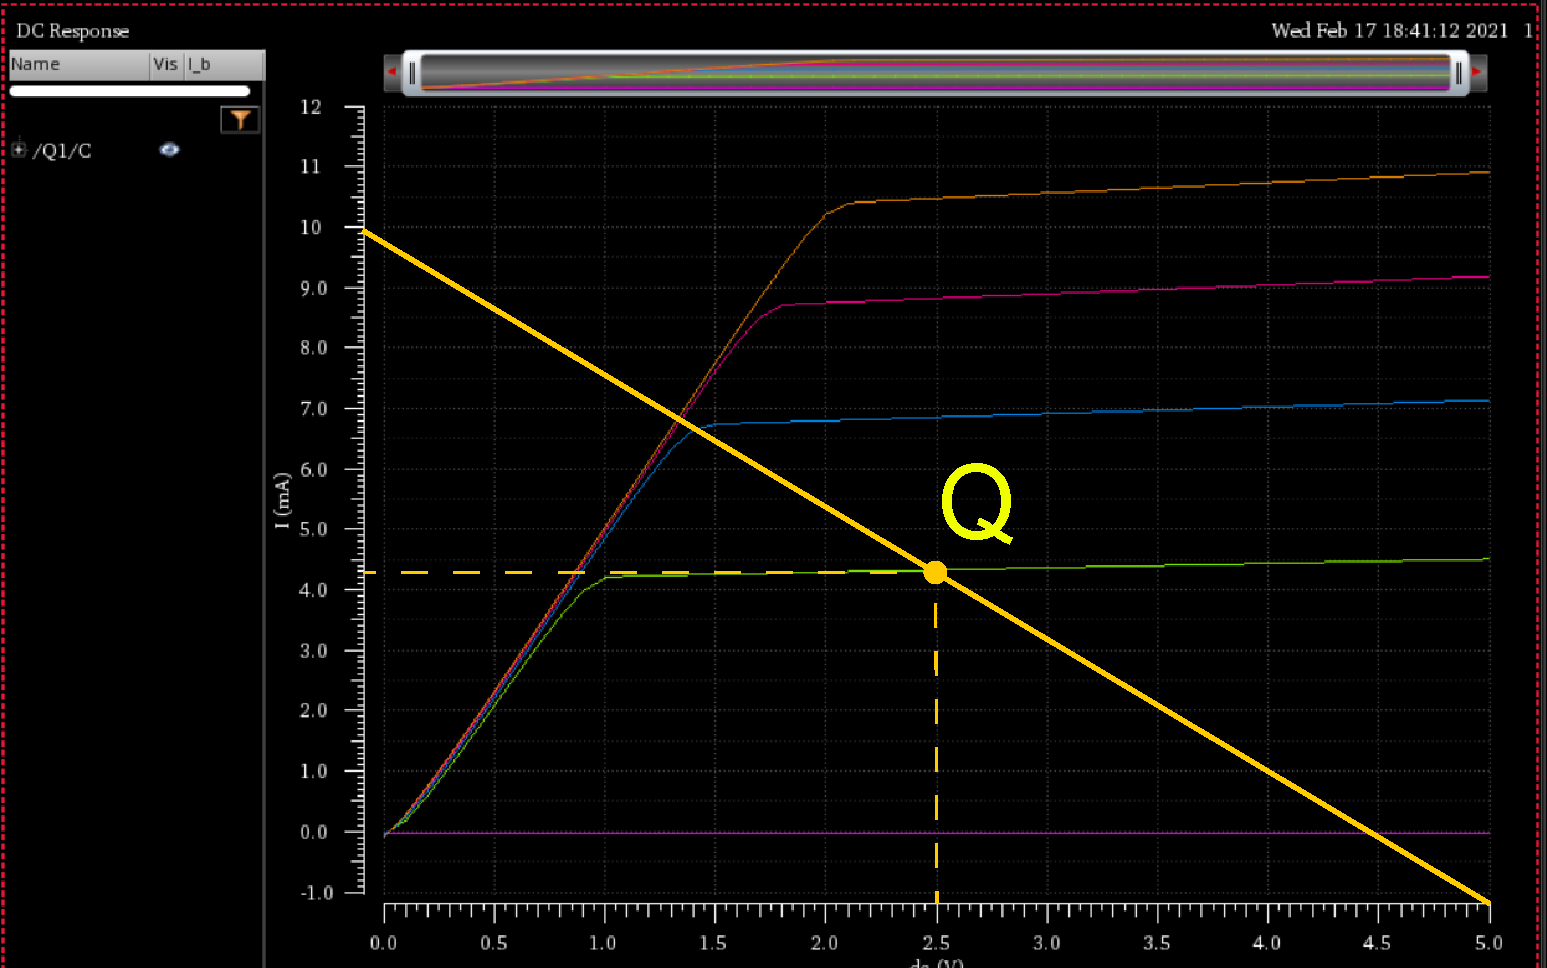
\includegraphics[width=0.7\linewidth]{1.png}}
	\caption{Схеми комбінаційних пристроїв, які досліджуються в лабораторній роботі.}
	\label{ris1}
\end{figure}


\begin{center}
\textbf{Робоче завдання}
\end{center}
Встановити лабораторний стенд «ДИСКРЕТ‑М» в режим «ЛАБ6» за допомогою перемикача лабораторних робіт, який знаходиться на задній панелі стенда. 
Включити кнопку «СЕТЬ».
Встановити на генераторі Г5-54 частоту проходження імпульсів $f_{BX}$=100кГц. Основний імпульс (ОІ) позитивної полярності амплітудою 5В, тривалістю $t_{1}$=3мкс з затримкою $t_{2}$=3,5мкс щодо синхроімпульса (СІ) подати на роз'єм «Ген.1». Синхроімпульс позитивної полярності амплітудою 5В подати на роз'єм «Ген.2», використовувати зовнішню синхронізацію осцилографа сигналом КТ6.\\
\textbf{I}.  Дослідити роботу дешифратора.\\
Зняти та побудувати часові діаграми: КТ2, КТ3, КТ4, КТ5, КТ6, КТ9, КТ8 та КТ7.\\
\textbf{II}.  Дослідити роботу мультиплексора та демультиплексора.\\
Зняти та побудувати часові діаграми: КТ2, КТ3, КТ4, КТ5, КТ6, КТ9, КТ8, КТ7, КТ1, КТ12, КТ11, КТ10, КТ13, КТ16, КТ15, КТ14.
Код, який задається за допомогою перемикачів П1, П2 та П3 задається викладачем на початку заняття.\\  
Звернути увагу, що адресними входами мультиплексора є входи КТ9, КТ8, КТ7 та КТ1.

\begin{center}
\textbf{Виконання завдання}
\end{center}
 \begin{figure}[h!]
	\center{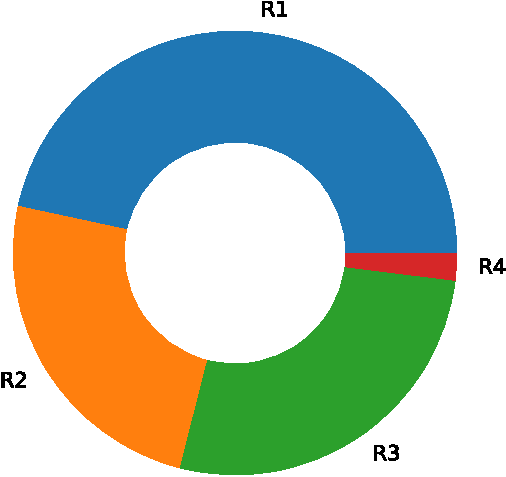
\includegraphics[width=0.8\linewidth]{2.png}}
	\caption{Часові діаграми, які демонструють особливості роботи дешифратора, мультиплексора та демультиплексора.}
	\label{ris2}
\end{figure}

\clearpage 
\newpage
\begin{center}
\textbf{\fbox{Висновок}}
\end{center}

В ході лабораторної роботи було досліджено задану систему, що містить дешифратор, мультиплексор та демультиплексор. За отриманими графіками
можна судити про принцип роботи логічних компонентів, що були використані та їх вплив на початковий сигнал генератора. Про деякі з компонентів окремо, дешифратор(КТ7, КТ8, КТ9 ...) бачимо високий сигнал там, де вiдсутнi  сигнали $\Rightarrow$ КТ9, видає високий сигнал, таким чином ми бачимо що iмпульси вiдсутнi, так само КТ8 та КТ7, вони реєструють 1 та 2 вiдповiдно, виводячи високий сигнал. Демультиплексор, тут при появi нульового iмпульсу та передаваючого  маємо низький сигнал при нульовому iмпульсi,так само пояснються дiаграми для КТ15 та КТ14 , до яких пiд’єднанi iнформацiйнi шини 1 та 2 з дешифратора та вихiд мультиплексора. 









\end{document}